\chapter{Human affect understanding through context fusion}
In the previous chapter, we explored how visual scene context information can be extracted from multimodal sources, especially media content, by utilizing large-scale pretrained external multimodal models. In this chapter, we will investigate the usage of contextual signals for instance-level multimodal content understanding. We consider instance-level multimodal content understanding along the granularity of individual persons and their perceived affective states in the scene. 
\section{Human affect understanding}
 There has been increased interest in understanding the affective processes associated with various facets of human emotions \cite{dukes2021}. An integral part of affective understanding is the ability to infer expressions of human emotions from various sources like images \cite{AICA}, speech \cite{speechemo}, and language use \cite{Poria2019EmotionRI}, as seen in Fig \ref{}. Affect recognition systems have enabled multiple human-centered applications, notably in healthcare (depression detection \cite{depressiondetection}, autism-spectrum diagnosis \cite{autismguha}) and learning \cite{savchecnkoengagement}).

\begin{figure}[h!]
    \centering
    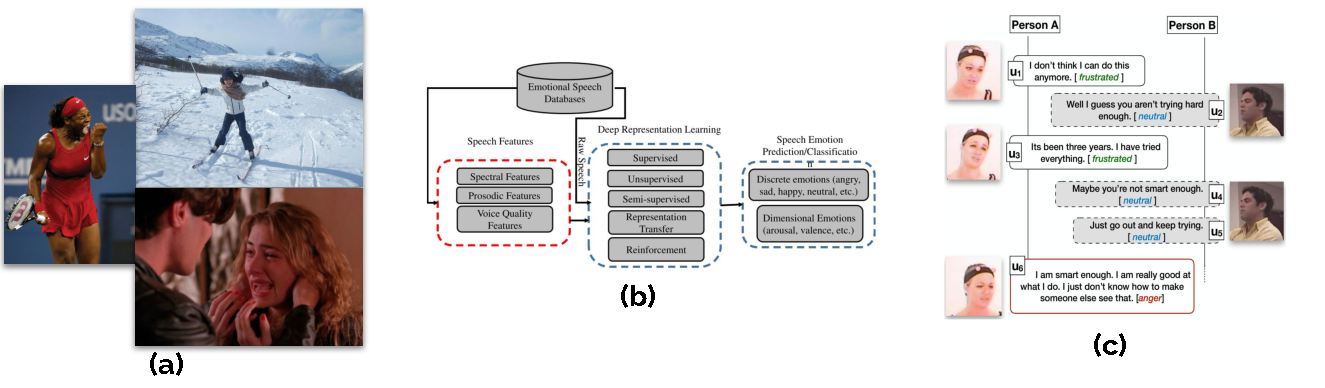
\includegraphics[width=\textwidth]{figures/emotion_overview.pdf}
    \caption{Overview of sources associated with different modalities (mentioned in brackets). \textbf{(a)} images (\textbf{visual}) \textbf{(b)} speech (\textbf{audio}) \textbf{(c)} language (\textbf{language}).}
    \label{emotion overview}
\end{figure}

 
\subsection{Facial expression - Is it the complete picture?}

Affect recognition from images has primarily focused on facial expressions \cite{DFEW,Mollahosseini2019AffectNetAD} along a fixed set of categories. Moreover, facial expression-based methods typically consider crops of a single face, which might provide ambiguous signals for classifying perceived emotions. An example where the face crop doesn't provide a complete picture for decoding the human affective state is shown in Fig \ref{face crop}. In Fig \ref{face crop} (a), we can see that the face crop for the child indicates a perceived affective state of surprise. But after including the entire global scene context, it can be inferred that the child is feeling happy and excited due to the event, i.e., birthday.
Further, in Fig \ref{face crop} (b), we can see that the face crop provides a noisy and incomplete picture. After taking into account the surrounding context that involves a troublesome situation of flooding, it can be assumed that the woman is feeling annoyed. Hence, in this work, we aim to include contextual cues from the visual scene and foreground interactions that contribute to the perception of affective state.

\begin{figure}[h!]
    \centering
    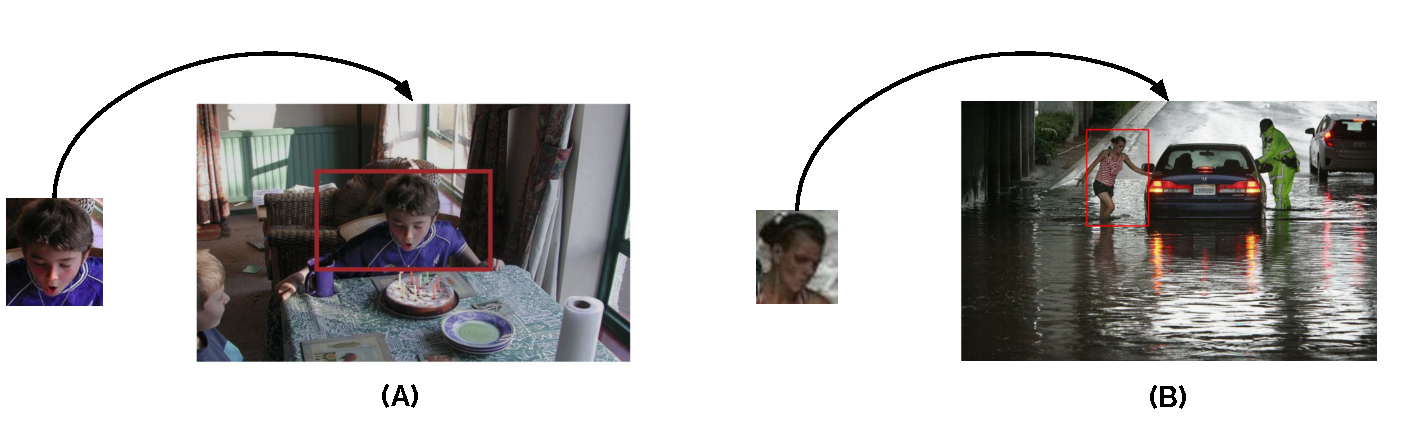
\includegraphics[width=\textwidth]{figures/face_crop_drawings.pdf}
    \caption{Examples from \textbf{EMOTIC} dataset where \textbf{(a)} face crop only provides an incomplete picture \textbf{(b)} face crop provides a noisy signal }
    \label{face crop}
\end{figure}


\section{Role of context in affect perception}
\textbf{Context in Emotion Perception:} The role of context extraneous to a person (beyond their traits and behavior) in the perception of their expressed emotion has been studied from the perspective of scenes \cite{BarretEmotionPerception}, and cultures \cite{Masuda2008PlacingTF}. In \cite{Dudzik2019ContextIH}, the perceivable-encoding context and the prior knowledge available with the perceivers are reported as the major sources of context for influencing emotion perception.  Situational context, like reactions from other people, has been considered in \cite{Wieser2012FacesIC} as a means to decode emotional states of persons in consideration.\\
\textbf{Context-based image datasets:} Image-based emotion recognition datasets like AffectNet \cite{AffectNet}, FER \cite{BarsoumICMI2016}, DFEW \cite{DFEW} primarily focus on signals encoded in facial expressions. Since emotion perception depends on where the facial configuration is present, datasets like EMOTIC \cite{kostiPAMI} and CAER \cite{CAER-S} have been proposed to incorporate contextual information in terms of visual scenes and social interactions. In the case of EMOTIC, annotators have marked person instances in unconstrained environments with apparent emotional states based on the existing scene context. However, the annotation process in CAER revolves around TV shows with primary focus on interactions-driven context. 
\\
\textbf{Context modeling approaches:} 
\cite{kostiPAMI,CAER-S} explore context modeling in terms of dual stream models for processing body and whole image streams. \cite{CAGER} also uses a dual stream network with context stream, modeled using an affective graph composed of region proposals.\cite{Mittal2020EmotiConCM} uses depth and pose as additional contextual signals with existing streams like scene, face for predicting person-specific emotion.
\cite{pikoulis2021leveraging} explores contextual modeling in short movie clips by considering scene and action characteristics along with body (including face) based signals. In contrast, our approach uses natural language descriptions to describe the foreground context along with scene and person-specific streams.
\\
\textbf{Multimodal vision-language models:} Vision language (VLN) models like OFA \cite{wang2022ofa}, VL-T5 \cite{cho2021vlt5}, ALBEF \cite{ALBEF} are pretrained on large-scale image-text pairs curated from the web, thus enabling its usage in diverse tasks like image captioning, retrieval, visual-question answering etc. In our formulation, we harness the capabilities of VLN models to generate descriptive captions since they contain condensed descriptions of the foreground context in terms of entities, including persons.


\section{Human affect understanding framework}

\begin{figure}[h!]
    \centering
    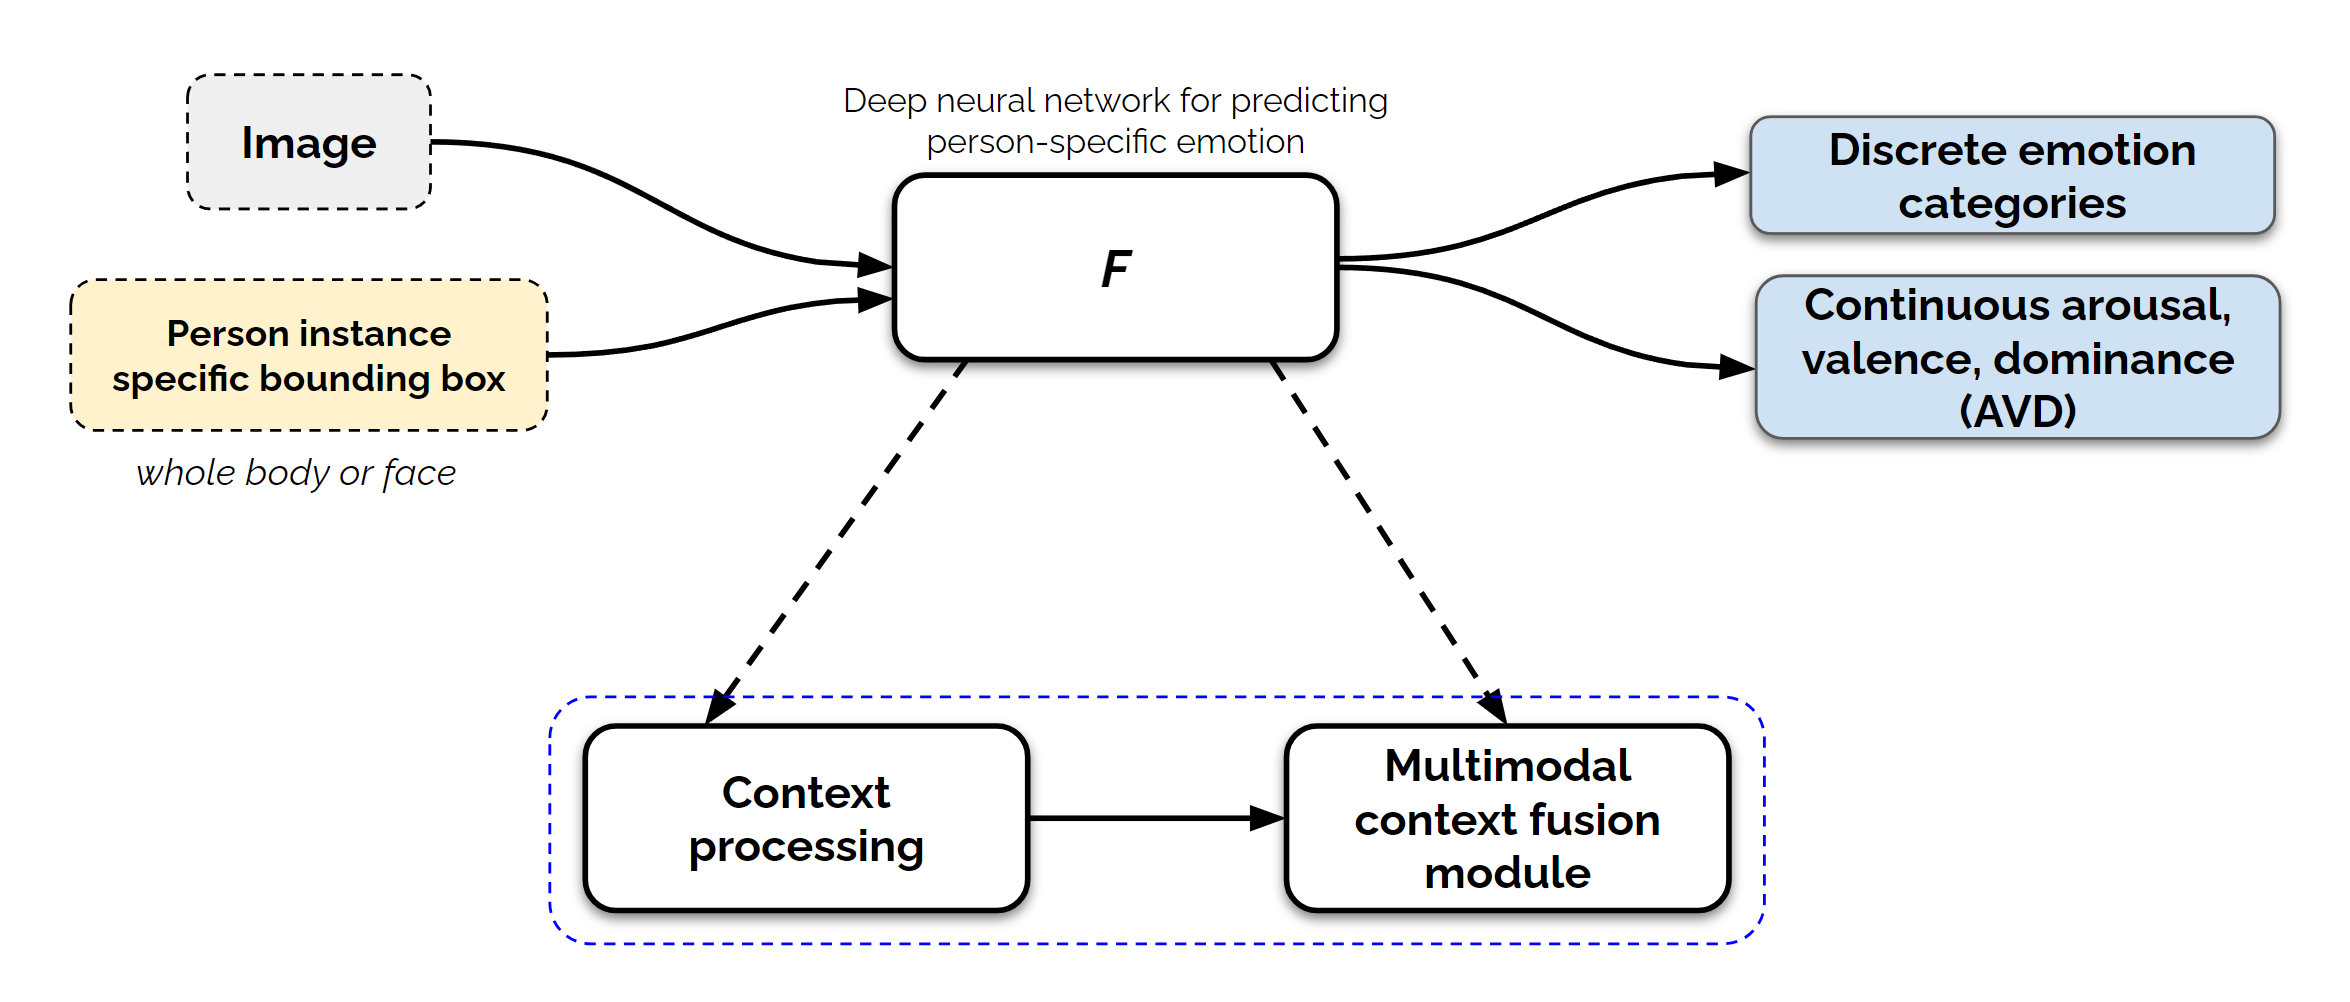
\includegraphics[width=\textwidth]{figures/human_affect_understanding.png}
    \caption{Outline of the human affect understanding framework }
    \label{human affect understanding}
\end{figure}

As seen in fig \ref{human affect understanding}, the human affect understanding relies on a neural network-based framework \textbf{\textit{F}} that consists of two segments: \textbf{Context processing} and \textbf{Multimodal context fusion module}. In terms of formal definition, given an image $I$ and a person-specific context in the form of bounding box $[x,y,w,h]$, the task is to predict the emotional state $p$ associated with a person as $p_{disc}, p_{cont} = F(I,[x,y,w,h])$. $p_{disc}$ and $p_{cont}$ refer to the predicted set of discrete emotion categories and continuous arousal, valence, and dominance values, respectively.

\section{Contextual processing - Multimodality:}

We extract contextual information through multiple modalities and use them for our subsequent instance-level content understanding task, i.e., affect estimation of a person. The outline of the context processing through different modalities is shown in Fig \ref{context_extraction}.

\begin{figure}
    \centering
    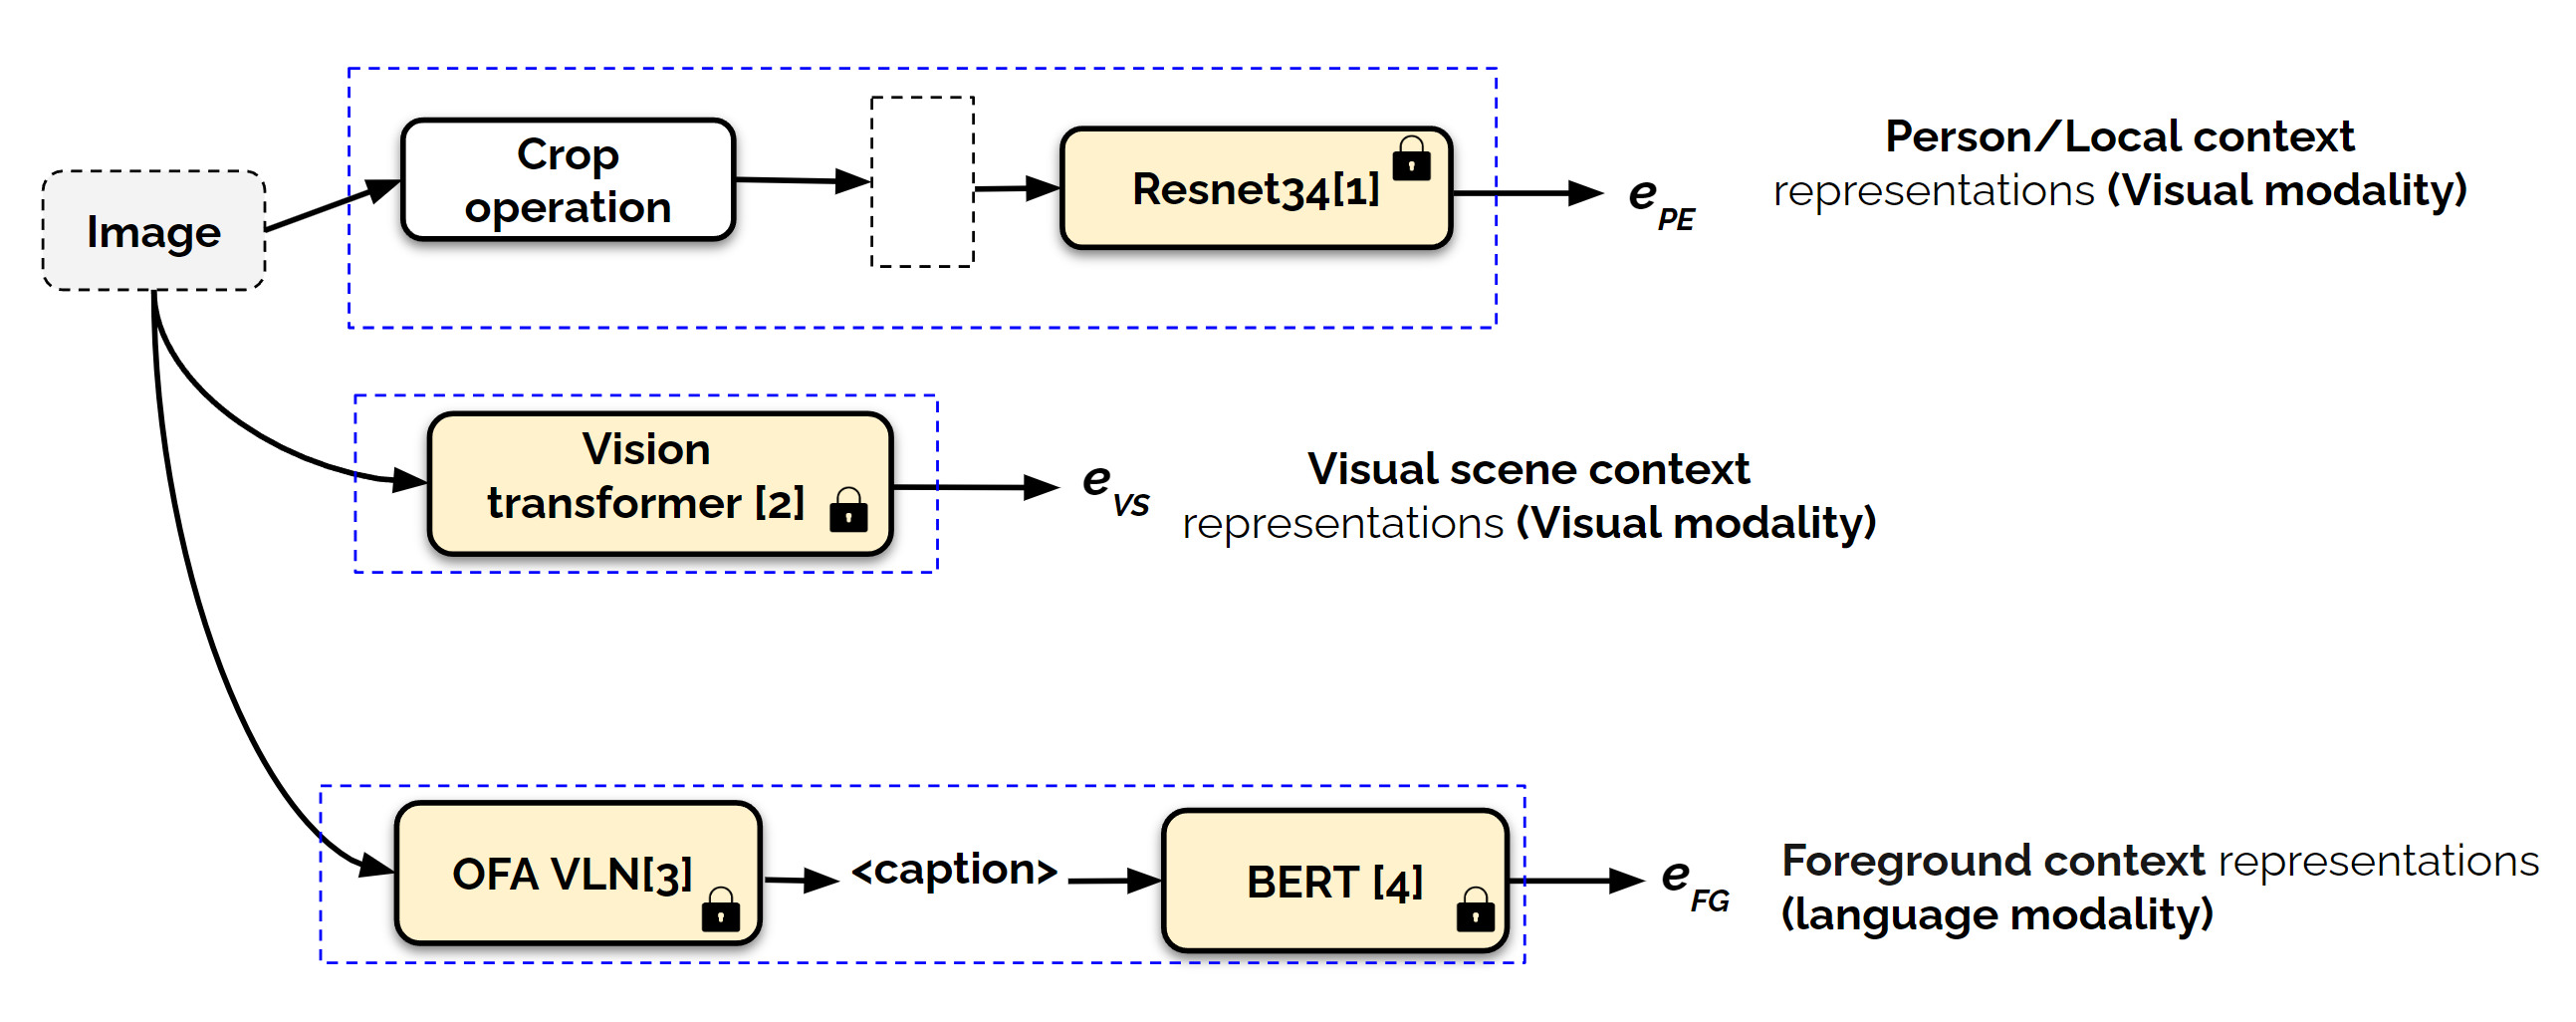
\includegraphics[width=\textwidth]{figures/context_extraction_multimodality.png}
    \caption{Outline of context processing through various modalities}
    \label{context_extraction}
\end{figure}
In the following subsections, we outline the process associated with the extraction of context information from the image.

\subsection{Visual scene context}
The underlying visual scene ($VS$) (e.g.,  kitchen, bar, football field etc) plays a role in influencing the emotional state of a person. Here we use a ViT \cite{Dosovitskiy2021AnII} model ($f_{VS}$) finetuned on Places365 \cite{zhou2017places} as the backbone network for extracting visual scene representations ($e_{VS}$) from $I$.
\subsection{Person-specific context}
The person-specific context is extracted using a whole-body or facial bounding box, denoted by $[x,y,w,h]$ from image $I$. The cropped person instance is passed through a person encoder ($f_{PE}$), i.e., Resnet34~\cite{He2016DeepRL} for extracting person-centric representations ($e_{PE}$). 
\subsection{Language-driven foreground context}
 Natural language description of image $I$ provides foreground (FG) context in terms of entities, including persons and their interactions. We use a 12-layer transformer encoder-decoder model $OFA_{large}$ \cite{wang2022ofa} as $f_{expert}$ to extract the foreground-specific captions for image $I$. For extracting text representations ($e_{FG}$) of the captions, we use BERT's \cite{Devlin2019BERT} pretrained encoder ($f_{FG}$) from HuggingFace \cite{wolf-etal-2020-transformers}.
\section{Multimodal context fusion module}

We propose a multimodal context fusion module to process the interaction of the person instance with foreground and background (visual scene).
\begin{figure}[h!]
    \centering
    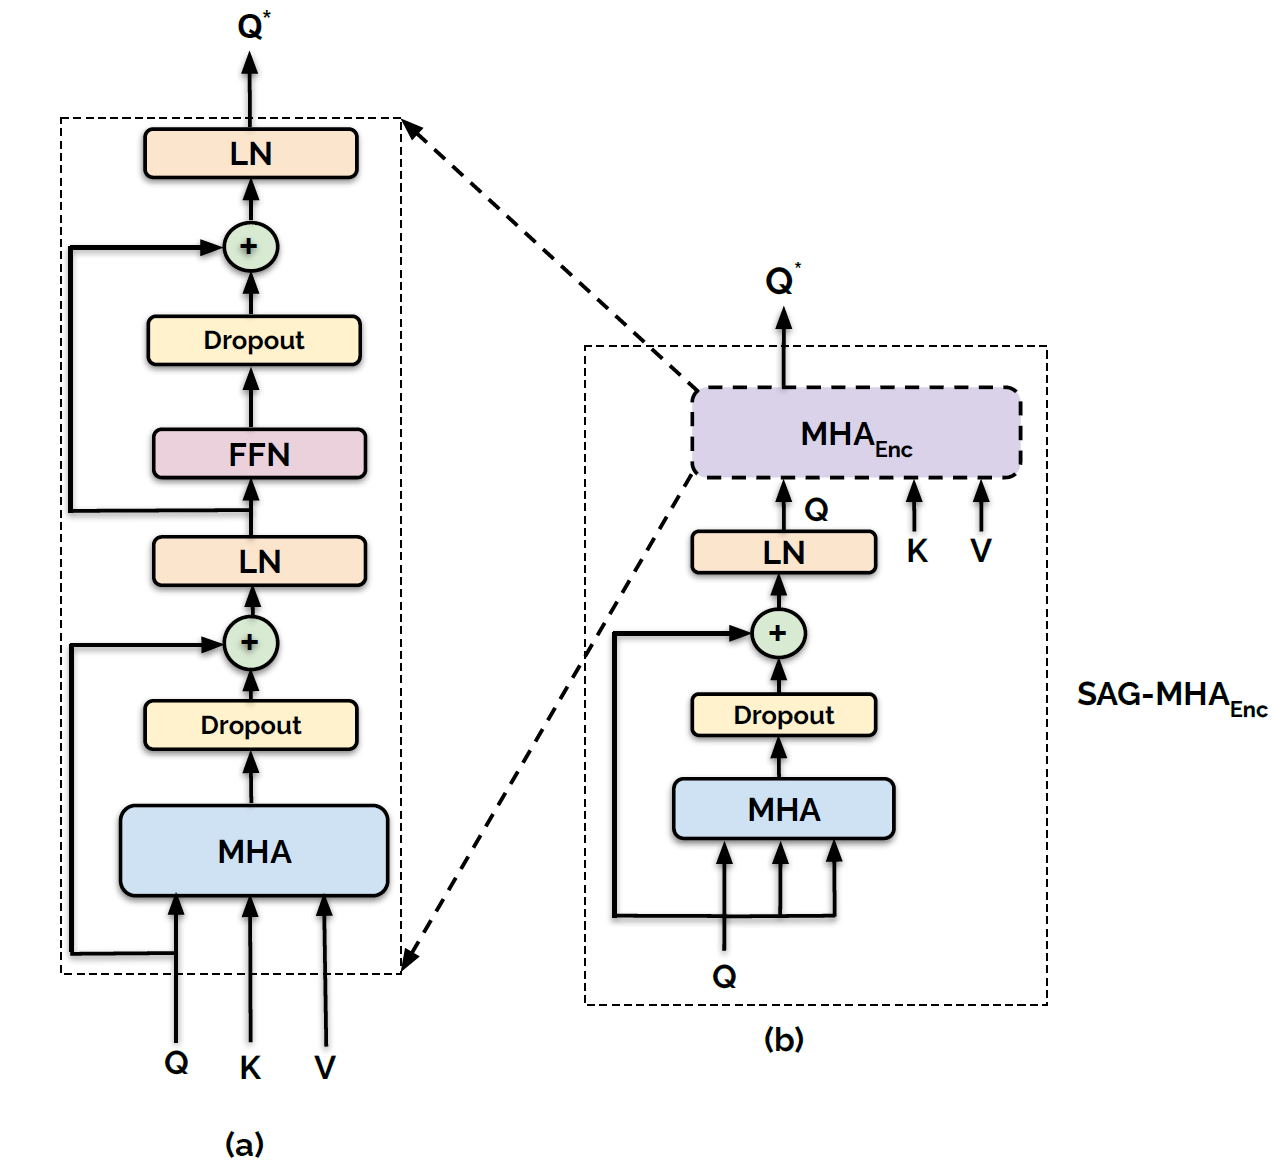
\includegraphics[width=0.7\textwidth]{figures/SAG_MHA.png}
    \caption{Outline of (a) MHA\textsubscript{enc} (b) SAG-MHA\textsubscript{enc} layers. \textbf{LN}: Layer Norm, \textbf{FFN}: Feedforward network, \textbf{MHA:} Multihead attention, \textbf{SAG:} Self Attention Augmented}
    \label{encoder block}
\end{figure}
The multimodal context fusion module is composed of two parallel streams, associated with foreground and visual scene-based contexts. The basic operation in individual streams is a cross-modal encoder block CM\textsubscript{enc} composed of L encoder layers. As shown in Fig \ref{encoder block}, we consider two designs for the encoder layer i.e., MHA\textsubscript{enc} and SAG-MHA\textsubscript{enc}.  
The set of operations in encoder MHA\textsubscript{enc} layer for query ($Q$), key ($K$) and value ($V$) representations are listed as follows:
\begin{equation} \label{MHAEnc operation}
\begin{split}
 Q^{'} & = LN(Q + \text{Dropout}(MHA(Q,K,V))) \\ 
Q^{*} & =LN(\text{Dropout}(FFN(Q^{'}))+Q^{'})
\end{split}
\end{equation}
Here $MHA$, $LN$ and $FFN$ refer to Multi-head attention, layer-norm operation and feed-forward neural network respectively. The SAG-MHA\textsubscript{enc} layer consists of a multi-head attention based transformation of the query representations followed by input to the MHA\textsubscript{enc} layer. The design of SAG-MHA\textsubscript{enc} is inspired from multimodal co-attention layer proposed in \cite{yu2019mcan} for visual question answering task.
\begin{equation} \label{SAG-MHAEnc operation}
\begin{split}
 Q^{'} & = LN(Q + \text{Dropout}(MHA(Q,Q,Q))) \\ 
Q^{*} & = MHA_{enc}( Q^{'},K,V) 
\end{split}
\end{equation}
In CM\textsubscript{enc}, the output from the $i$th encoder layer $Enc_{i}$ is passed as query ($Q$) to the subsequent layer with the key ($K$) and value ($V$) remaining the same. Here, $Enc_{i}$ layer can be either MHA\textsubscript{enc} or SAG-MHA\textsubscript{enc}.
\begin{equation} \label{encoder layer operation}
\begin{split}
    Q_{i}&=Enc_{i}(Q_{i-1},K,V) \     i > 0 \\
    Q_{0} &=Enc_{0}(Q,K,V)
\end{split}
\end{equation}
We use separate CM\textsubscript{enc} blocks for processing the foreground and visual scene-guided context streams. MCF (MHA\textsubscript{enc}) and MCF (SAG-MHA\textsubscript{enc}) consists of 4 MHA\textsubscript{enc} layers (8 heads and hidden dimension=512) and 3 SAG-MHA\textsubscript{enc} layers (8 heads and hidden dimension=768) in the CM\textsubscript{enc} blocks respectively.

\begin{figure}[h!]
    \centering
    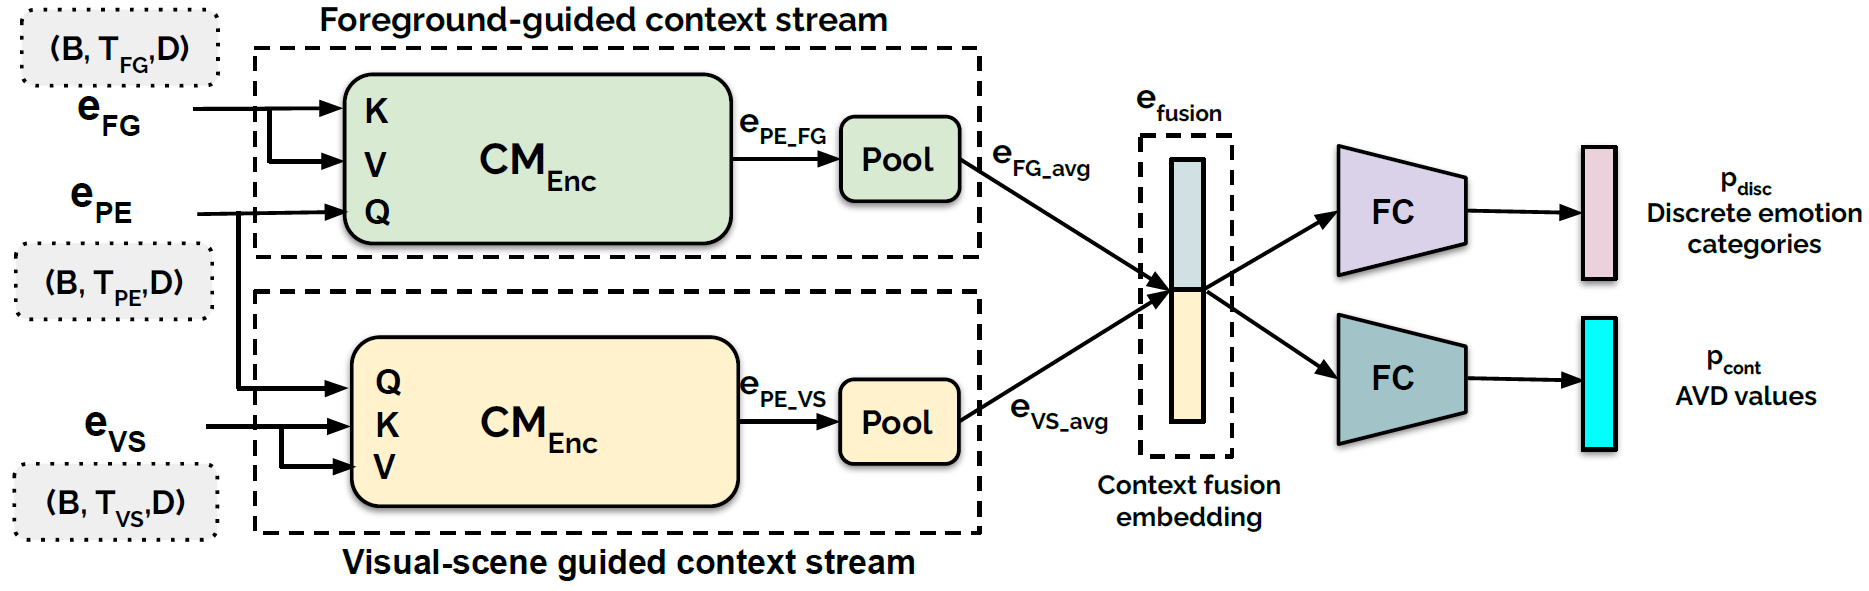
\includegraphics[width=\columnwidth]{figures/MCF_module_updated.png}
    \caption{Outline of the $MCF$ module. Separate CM\textsubscript{enc} blocks are used to model the foreground and visual scene context streams. $B$: Batch size. $D$: Hidden dimension. Token length of $T_{FG}$: text representations, $T_{PE}$: person representations, $T_{VS}$: visual scene representations. AVD: Arousal, Valence, Dominance
    }
    \label{mcf module}
\end{figure}
The details of the respective context-guided streams are listed as follows:\\
\textbf{\underline{Foreground-guided context stream:}} We use $e_{PE}$ as query ($Q$) and $e_{FG}$ as key and value inputs to the CM\textsubscript{enc} encoder.\\
\textbf{\underline{Visual-scene guided context stream:}} Similar to the foreground-guided context stream, we use $e_{PE}$ as query ($Q$) and $e_{VS}$ as key and value inputs to the CM\textsubscript{enc} encoder.\\
\textbf{\underline{Context fusion:}}
The outputs from the context-guided streams i.e., $e_{PE\_{FG}}$ and $e_{PE\_{VS}}$ are average pooled and concatenated to obtain a fused embedding as: $e_{fusion}=[e_{FG\_{avg}};e_{VS\_{avg}}]$
\section{Experiments}
\subsection{Emotic}

We use a non-intersecting split of 13584 and 4389 images for training and validation. For testing we use the publicly available split of 5108 images. For joint prediction of 26 discrete emotion classes and the continuous-valued AVD ratings, we use multiple fully-connected (FC) heads in the $MCF$ module with $e_{fusion}$ as input (Fig \ref{mcf module}). The person specific instance in each image is defined by the ground truth person box. We do not consider face as a part of person-specific context since approx 25\% of images do not have visible faces. \\
For training $MCF$ with MHA\textsubscript{enc} and SAG-MHA\textsubscript{enc} layers, we use AdamW \cite{AdamW} (\textit{lr=2e-5}) and Adam \cite{Adam} (\textit{lr=2e-4,  exp($\gamma$=0.90)}) with batch sizes 32 and 64 respectively. \footnote{exp is exponential scheduler \label{note1}}. We use SGD(\textit{lr=1e-2, exp($\gamma$=0.90)}) with a batch size of 64 while training the person-crop only Resnet34 model ($PO_{R34}$) in Table \ref{ablationemotic}. For training all the models associated with EMOTIC, we use a weighted combination of binary-cross entropy (BCE) and mean squared error (MSE) losses.
\begin{equation}
Loss =\lambda_{1} BCE(p_{disc},y_{disc}) + \lambda_{2} MSE(p_{cont},y_{cont})
\end{equation}
Here $y_{disc}$ and $y_{cont}$ refer to ground truth discrete emotion labels and continuous arousal valence dominance ratings. The optimal weights $\lambda_{1}$ and $\lambda_{2}$ are tuned using the validation split. 

\subsection{CAER-S}

We use a non-intersecting split of 39099 and 9769 video frames across 79 TV shows for training and validation. For testing, we use the public split of 20913 video frames. Since face is a dominant signal for persons in TV shows, we use MTCNN \cite{MTCNN} \footnote{https://github.com/timesler/facenet-pytorch} to obtain face crops. We have a single fully connected (FC) head with $e_{fusion}$ as input for predicting 7 discrete emotion classes. \\
For training $MCF$ with MHA\textsubscript{enc} and SAG-MHA\textsubscript{enc} layers, we use Adam (\textit{lr=2e-4, exp($\gamma$=0.90)}) with a batch size of 64. We use Adam (\textit{lr=1e-4, exp($\gamma$=0.75)}) with a batch size of 64 while training the face-crop only Resnet34 model ($FO_{R34}$) in Table \ref{ablationCAER-S}. For training all the models associated with CAER-S, we use multi-class cross-entropy loss.
\\
We conduct our experiments using the Pytorch \cite{Paszke2019PyTorchAI} library. We set the maximum sequence length $T_{FG}$ as 512 for the captions (Fig \ref{mcf module}). For visual scene and person representations, we use $T_{VS}=197$ and $T_{PE}=49$, respectively.

\section{Results}

\subsection{Emotic}

\subsubsection{Context modeling variations}
\begin{table}[h!]
\centering
\begin{tabular}{|c|c|c|c|}
\hline
\textbf{Model}                      & \textbf{mAP}            & $\mathbf{\lambda_{1}}$ & $\mathbf{\lambda_{2}}$ \\ \hline
PO\textsubscript{R34}                  & 23.46 (0.006)           & 0.95                   & 0.05               \\ \hline
PO\textsubscript{R34} + VS +LF & 25.53 (0.025)           & 0.6                    & 0.4                \\ \hline
CM\textsubscript{Enc} (MHA\textsubscript{enc} + VS)        & 27.37 (0.004)           & 0.5                    & 0.5                \\ \hline
\textbf{MCF (MHA\textsubscript{enc})}               & \textbf{29.53 (0.001)} & \textbf{0.8}           & \textbf{0.2}       \\ \hline
\end{tabular}
\caption{Associated models and different context streams for EMOTIC. \textbf{PO}: Person-only model, \textbf{R34}: Resnet34 fully fine-tuned, \textbf{VS}: Visual scene, \textbf{cls:} cls token, \textbf{LF:} Late fusion, $\mathbf{\lambda_{1}}$: BCE weight, $\mathbf{\lambda_{2}}$: MSE weight. Average of runs with 5 random seeds reported with standard deviation for the models}
\label{ablationemotic}
\end{table}
We analyze the importance of different input context streams and associated models in EMOTIC. From Table~\ref{ablationemotic}, we can see that the Resnet34 model ($PO_{R34}$) fully finetuned using person specific crops performs worst, thus indicating the need of additional contextual information. Inclusion of scene representation (cls token) from ViT pretrained on Places2 dataset with $PO_{R34}$ via late fusion (LF) improves the mAP to \textbf{25.53}. Freezing $PO_{R34}$ model followed by cross modal interaction through $CM_{enc}$ composed of MHA\textsubscript{enc} layers (visual-scene guided context stream in Fig.~\ref{ablationemotic}) further increases the mAP to \textbf{27.37}. Further we can see that fusion of both foreground and visual scene based context information through MCF (MHA\textsubscript{enc}) results in the best performance (\textbf{29.53}). For both CM\textsubscript{Enc} (MHA\textsubscript{enc} + VS) and MCF (MHA\textsubscript{enc}), we freeze the Resnet34 model for extracting representations from person crops. 

\subsubsection{Comparisons with state of the art}
We compare the performance of $MCF$ (Enc) under two settings where Enc refers to the encoder layer used i.e., MHA\textsubscript{enc} and SAG-MHA\textsubscript{enc} with existing methods in Table \ref{MHAEnc}. We can see that $MCF$ under both settings performs better than prior methods like  \cite{kostiPAMI}, \cite{CAGER}, and \cite{CAER-S} that rely on dual stream (person + whole image approach) and do not use explicit pose information. Furthermore, in contrast to previous methods, we consider language-driven foreground (captions) and visual scene contexts instead of end-to-end modeling of whole image-based information. For a fair comparison with \cite{Mittal2020EmotiConCM}, the current $MCF$ framework can be potentially expanded to include other person-specific streams like face and explicit pose information.
\begin{table}[h!]
\centering
\begin{tabular}{|c|c|}
\hline

\textbf{Model}   & \textbf{mAP}   \\ \hline
Kosti et. al \cite{kostiPAMI} & 27.38          \\ \hline
Zhang et. al  \cite{CAGER}   & 28.42          \\ \hline
Lee et.al  \cite{CAER-S}      & 20.84          \\ \hline
\textbf{MCF (MHA\textsubscript{enc})}     & \textbf{29.53 (0.001)} \\ \hline
MCF (SAG-MHA\textsubscript{enc}) & 28.58 (0.003)  \\ \hline
EmotiCon \cite{Mittal2020EmotiConCM}       & 32.03          \\ \hline
\end{tabular}
\caption{Comparison of $MCF$ module with state of the art in EMOTIC (Test). \textbf{mAP:} mean average precision. Average of runs with 5 random seeds reported with standard deviation for $MCF$.}
\label{MHAEnc}
\end{table}
\subsection{CAER-S}
\subsubsection{Context modeling variations}
\begin{table}[h!]
\centering
\begin{tabular}{|c|c|c|}
\hline
\textbf{Model}  & \textbf{Accuracy} & \textbf{F1}  \\ \hline
FO\textsubscript{R34}          & 77.35 (0.002)     & 77.13 (0.002) \\ \hline
MCF (SAG-MHA\textsubscript{Enc}) & \textbf{79.63 (0.003)}     & \textbf{79.36 (0.003)} \\ \hline
MCF (MHA\textsubscript{Enc})     & 76.89 (0.003)      & 76.74 (0.002) \\ \hline
\end{tabular}
\caption{Associated models and different context streams for CAER-S. \textbf{FO}: Face-only model, \textbf{R34}: Resnet-34 fully fine-tuned, Average of runs with 5 random seeds reported with standard deviation for the models}
\label{ablationCAER-S}
\end{table}

For CAER-S, we can see from Table \ref{ablationCAER-S} that inclusion of SAG-MHA\textsubscript{enc} layer instead of MHA\textsubscript{enc} improves the accuracy from \textbf{76.89} to \textbf{79.63}.  This can be attributed to the self-attention based augmentation operation for the query features i.e. face representations from Resnet34 in SAG-MHA\textsubscript{enc} layer (Fig \ref{encoder block}). For both MCF (MHA\textsubscript{enc}) and MCF (SAG-MHA\textsubscript{enc}), we finetune the Resnet34 model completely with $MCF$ for extracting representations from face crops. 

\subsubsection{Comparisons with state of the art}

 \begin{table}[h!]
\centering
\begin{tabular}{|c|c|c|}
\hline
\textbf{Model}                               & \textbf{Accuracy}                      & \textbf{F1}                       \\ \hline
CAER-Net-S  \cite{CAER-S}                                & 73.51                             & \textbf{\_}                       \\ \hline
FO\textsubscript{R34}                                    & 77.35 (0.002)                     & 77.13 (0.002)                      \\ \hline
\multicolumn{1}{|l|}{MCF (SAG-MHA\textsubscript{enc})} & \multicolumn{1}{l|}{\textbf{79.63 (0.003)}} & \multicolumn{1}{l|}{\textbf{79.36 (0.003)}}\\ \hline
\end{tabular}
\caption{Comparison of $MCF$ module with state of the art in CAER-S (Test). \textbf{F1:} macro-F1, \textbf{FO:} Face only, \textbf{R34}: Resnet34 fully finetuned. Average of runs with 5 random seeds reported with standard deviation for $MCF$ and Resnet34.}
\label{MCFSAG}
\end{table}
From Table \ref{MCFSAG}, we can see that in CAER-S, a fully finetuned Resnet34 model trained on face crops ($FO_{R34}$) obtains a high accuracy of 77.35 since facial expressions provide dominant signals for emotion classification in TV shows. However, inclusion of both foreground context through captions and visual scene information in MCF (MHA\textsubscript{enc}) results in better performance (\textbf{79.63}) as compared to both $FO_{R34}$ and baseline attention fusion method CAER-Net-S. 

\subsection{Qualitative examples}
\begin{figure}[h!]
    \centering
    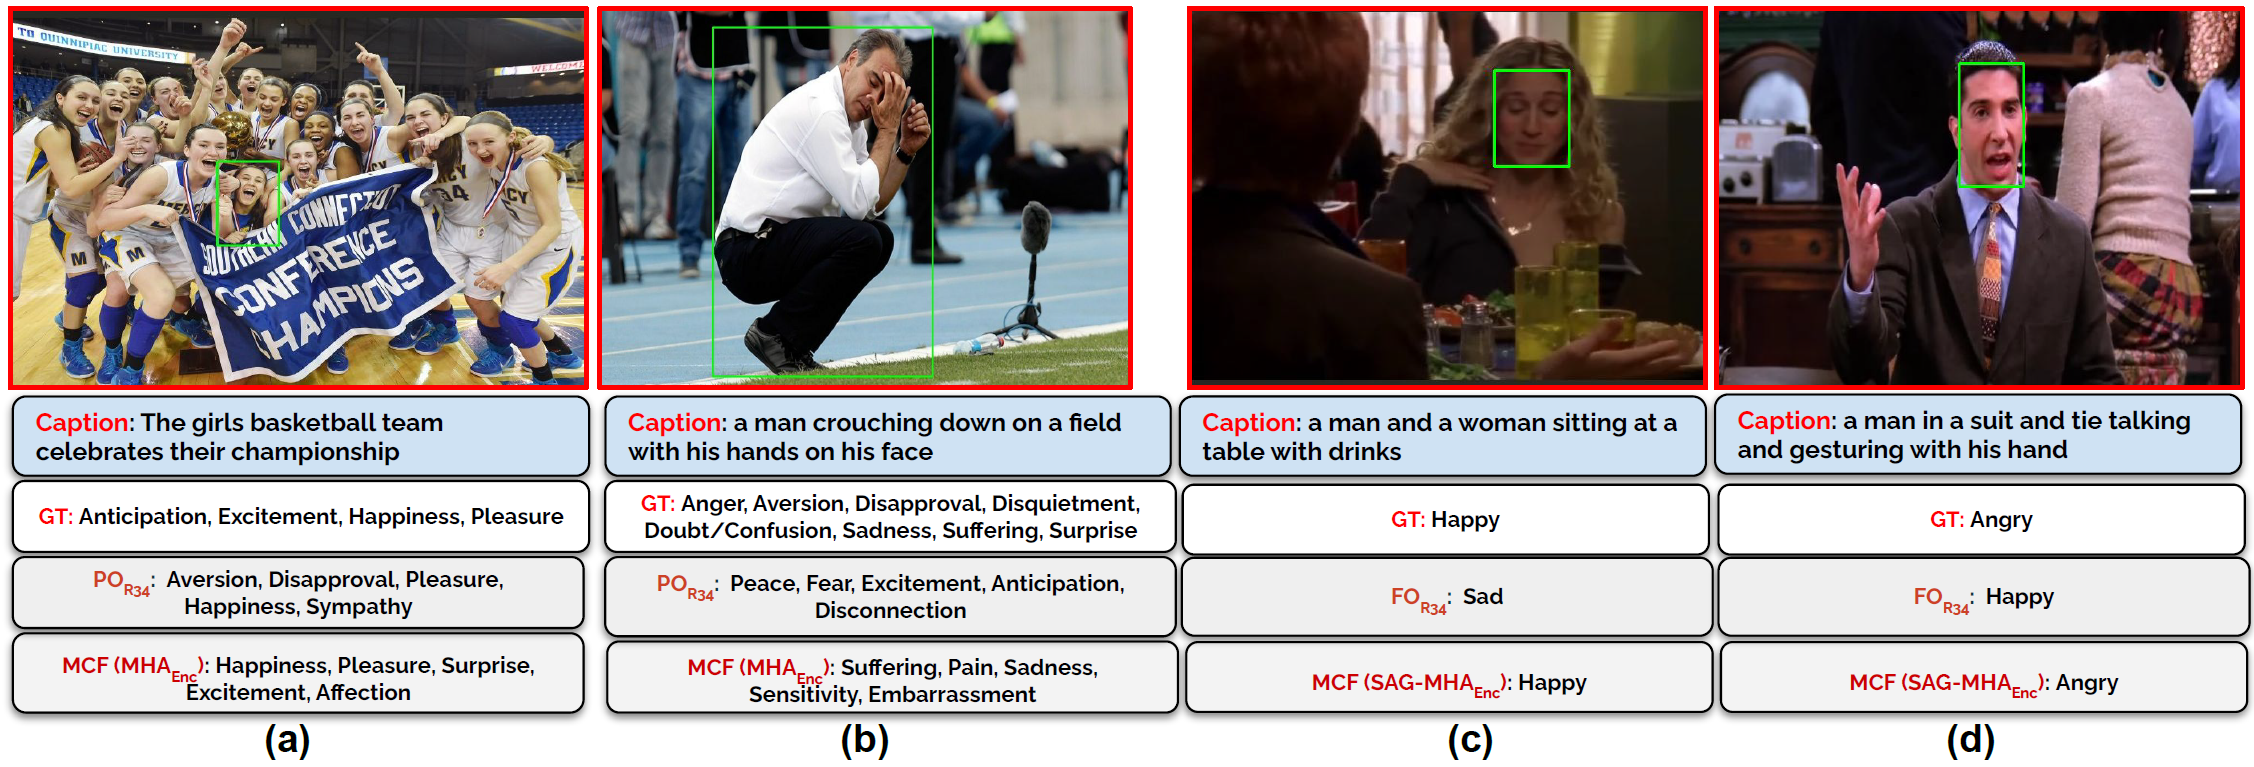
\includegraphics[width=\textwidth]{figures/EMOTIC_CAER_examples_updated.png}
    \caption{Examples (a) and (b) from EMOTIC showing comparisons between top-5 predictions of $PO_{R34}$ and MCF (MHA\textsubscript{enc}). Examples (c) and (d) from CAER-S showing comparisons between top predictions of $FO_{R34}$ and MCF (SAG-MHA\textsubscript{enc}) . $PO$: Person-only. $FO$: Face-only. $R_{34}$: Resnet34 fully finetuned. GT: Ground truth. Person or face instances marked by green bounding boxes}
    \label{qualfig}
\end{figure}

In Fig \ref{qualfig} (a) and (b), we can see that the inclusion of foreground context through captions like \textit{basketball team celebrating} and \textit{man crouching down with his hands on his face} results in consistent performance of MCF (MHA\textsubscript{enc}) as compared to $PO_{R34}$ (Resnet34 finetuned on person crops). Similarly, for TV shows in Fig \ref{qualfig} (c), while the face crop-based prediction from $FO_{R34}$ is \textbf{sad}, the inclusion of foreground context with visual scene information gives a correct prediction for MCF (SAG-MHA\textsubscript{enc}). In Fig \ref{qualfig} (d), the act of \textit{gesturing with hand} enables MCF (SAG-MHA\textsubscript{enc}) to make a correct prediction (\textbf{Angry}) as compared to $FO_{R34}$ (Resnet34 finetuned on face crops).

\section{Limitations}

\begin{figure}[h!]
\centering
\subfloat[]{%
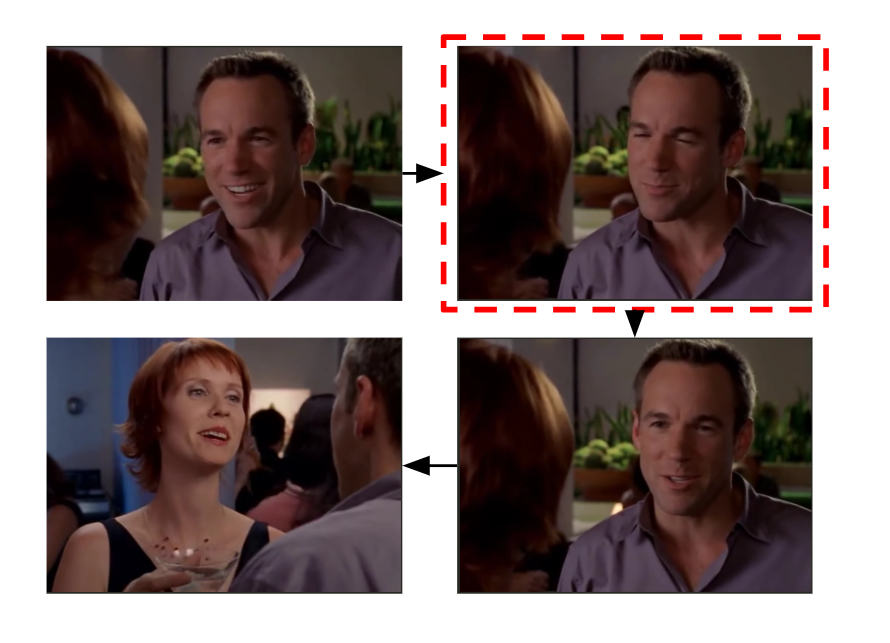
\includegraphics[width=0.5\textwidth]{figures/image_annotation.png}% 
\label{image annotation}
}
\subfloat[]{%
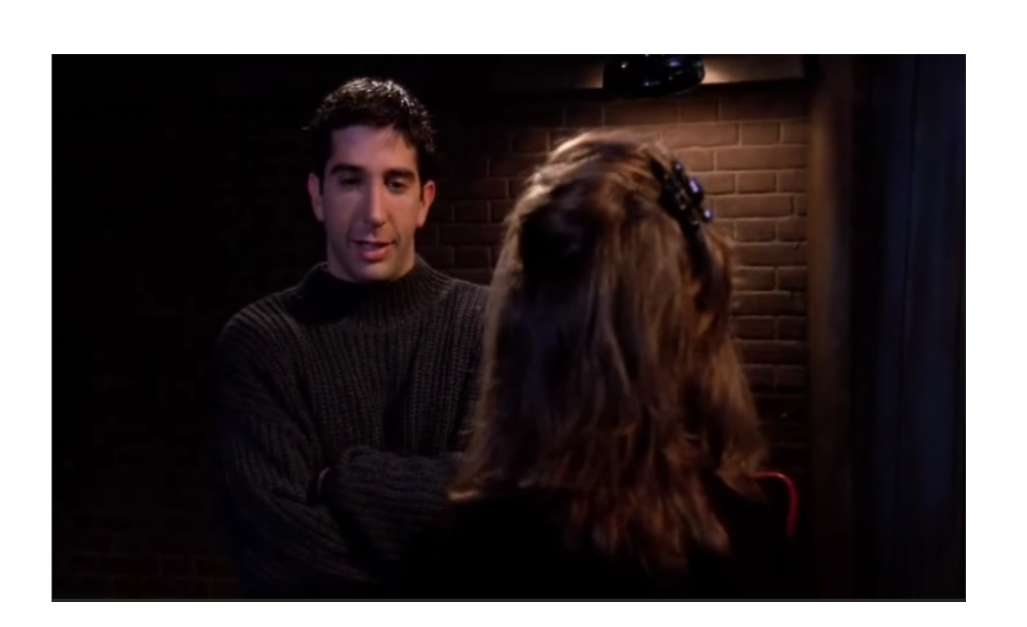
\includegraphics[width=0.5\textwidth]{figures/foreground_context.png}%
\label{foreground context}
}
\caption{(a) Lack of temporal information in image annotation (b) Incorrect foreground context predicted by OFA VLN \cite{wang2022ofa}: \textit{a man looking at a girl in a mirror}}
\label{temporal information and incorrect foreground}
\end{figure}

For image-based datasets like CAER-S, a lack of temporal information provides an ambiguous setting for marking the affective state of the person. For the red marked frame in \textbf{(a)}, it is difficult to infer that the person is feeling happy since the eyes and mouth are closed. However, if the interactions are taken into account, it can be seen that the person is feeling happy. Further, in the case of foreground context, OFA VLN provides the description: \textit{a man looking at a girl in a mirror}. This indicates that there are cases where the foreground context might not be captured correctly by pretrained vision language models.

% In this work, we explore the role of contextual information in estimating human emotions with respect to the domains of natural scenes (EMOTIC) and TV shows (CAER-S). Since multimodal-VLN models are pretrained on large-scale image-text pairs from the web, we utilize their capabilities to obtain foreground context information in terms of descriptive captions. Further, we propose a purely attention-based multimodal context fusion (MCF) module to combine person-specific information with the visual scene and foreground context representations. Future work involves the extension of the MCF module to include geometric aspects of person context including pose information and evaluation using media-centered data like movies and advertisements.

\section{Conclusion}

The major takeaways from the work are as follows:

\begin{itemize}

\item \textbf{Foreground context inclusion:} Foreground context in terms of activities/interactions with the environment can be captured through pretrained vision-language expert models.
 
\item \textbf{Role of context fusion:} Attention mechanisms guided by visual scene and foreground contexts with person information improve human affect understanding.

\item \textbf{Static viewpoint:} Images provide a static snapshot of the particular instant and do not consider the temporal context involved in the affective response.

\end{itemize}
